\documentclass[border=10pt]{standalone}

\usepackage{tikz}
\usepackage{tikzsymbols}
\usetikzlibrary{calc,patterns,shapes.geometric}

\def\centerarc[#1](#2)(#3:#4:#5){\draw[#1] ($(#2)+({#5*cos(#3)},{#5*sin(#3)})$) arc (#3:#4:#5);}

\begin{document}
	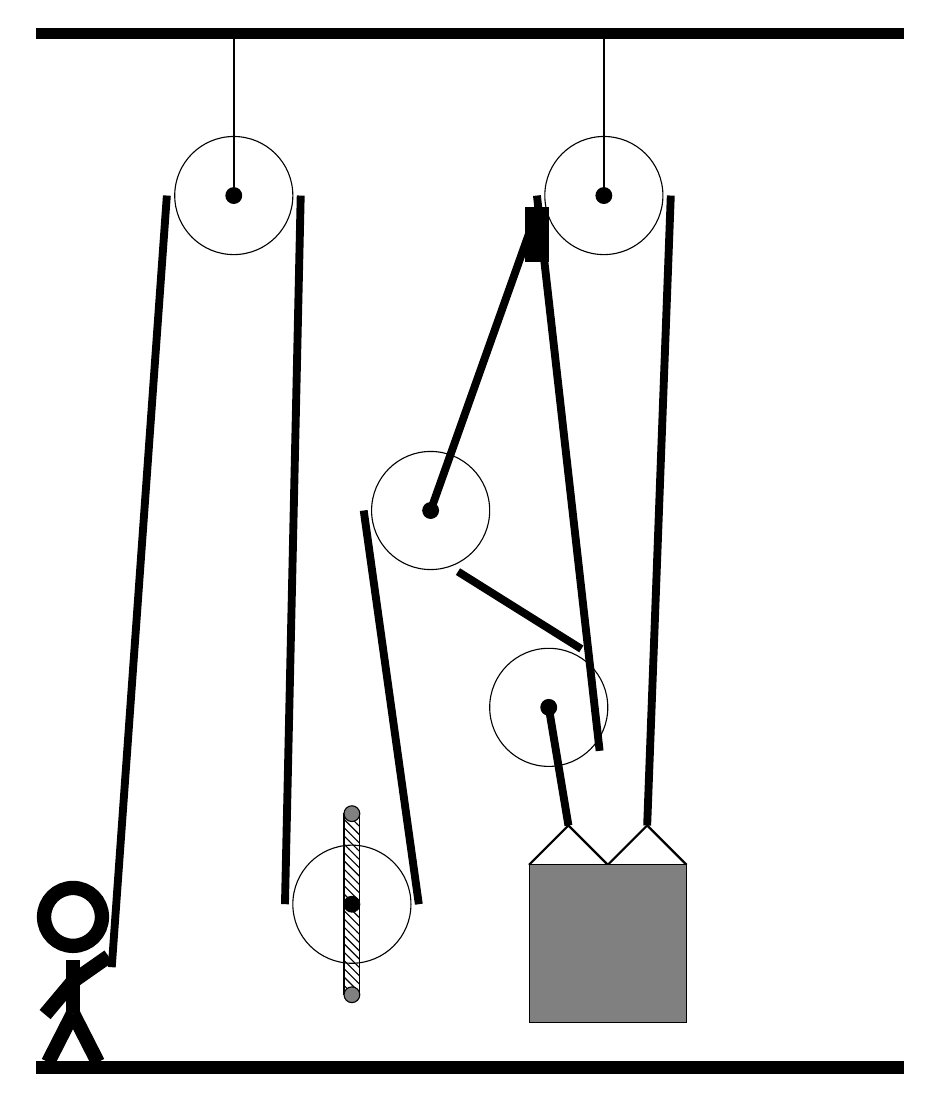
\begin{tikzpicture}
		%%%%% START %%%%%
		\draw[fill=black] (-6, 10) rectangle (5, 10.125);
		
		\draw (-1, 4.0) circle (0.75);
		\draw[fill=black] (-1, 4.0) circle (0.1);
		
		\draw (0.5, 1.5) circle (0.75);
		\draw[fill=black] (0.5, 1.5) circle (0.1);
		
		\draw (1.2, 8.0) circle (0.75);
		\draw[fill=black] (1.2, 8.0) circle (0.1);
		\draw[thick] (1.2, 8.0) -- (1.2, 10);
		
		\draw (-3.5, 8.0) circle (0.75);
		\draw[fill=black] (-3.5, 8.0) circle (0.1);
		\draw[thick] (-3.5, 8.0) -- (-3.5, 10);
		
		\draw (-2, -1.0) circle (0.75);
		\draw[fill=black] (-2, -1.0) circle (0.1);
		\draw[pattern=north west lines, pattern color=black] (-2.1, 0.15) rectangle (-1.9, -2.15);
		\draw[fill=black!50] (-2, 0.15) circle (0.1);
		\draw[fill=black!50] (-2, -2.15) circle (0.1);
		
		\draw[thick]  (0.25, -0.5) -- (0.75, 0.0) -- (1.25, -0.5) -- (1.75, 0.0) -- (2.25, -0.5);
		\draw[fill=black!50] (0.25, -0.5) rectangle (2.25, -2.5);
		\draw[line width=1mm] (-5.05, -1.8) -- (-4.35, 8.0);
		\centerarc[line width=1mm](-3.5, 8.0)(0:180:0.85);
		\draw[line width=1mm] (-2.65, 8.0) -- (-2.85, -1.0);
		\centerarc[line width=1mm](-2, -1.0)(180:360:0.85);
		\draw[line width=1mm] (-1.15, -1.0) -- (-1.85, 4.0);
		\draw[line width=1mm] (-1, 4.0) -- (0.35, 7.8);
		\draw[line width=1mm, fill=black](0.25, 7.2) rectangle (0.45, 7.8);
		\centerarc[line width=1mm](-1, 4.0)(-20:180:0.85);
		\draw[line width=1mm] (-0.653, 3.224) -- (0.914, 2.242);
		\centerarc[line width=1mm](0.5, 1.5)(160:380:0.85);
		\draw[line width=1mm] (1.146, 0.948) -- (0.35, 8.0);
		\draw[line width=1mm](0.5, 1.5) -- (0.75, 0.0);
		\centerarc[line width=1mm](1.2, 8.0)(0:180:0.85);
		\draw[line width=1mm] (2.05, 8.0) -- (1.75, 0.0);
		
		\node at (-5.5, -1.9) {\Strichmaxerl[10][50][35]};
		
		\draw[fill=black] (-6, -3) rectangle (5, -3.15);
		%%%%% END %%%%%
	\end{tikzpicture}
\end{document}